\section{Introduction}

With the development of computing technology, data storage usage continues to grow to high values. The development of data usage and storage is driven by the emergence of cloud computing technology, data needs for artificial intelligence training based on machine learning, and general improvement in data quality in files.

Along with this, the use of systems has become increasingly intensive. This intensive use creates a need for high resilience so that these systems can continue to operate, especially in facing the possibility of component failure and data loss \cite{weatherspoon2002erasure}. In this case, data redundancy solutions become very important. Traditionally, replication techniques are used to duplicate data to multiple nodes. However, with the growing need for data in operations, this approach consumes increasingly large storage capacity and significantly increases operational costs.

Another solution to address these failures is erasure coding. With the application of erasure coding, data storage requirements can be reduced while maintaining data integrity and resilience, especially in distributed system environments using multiple devices simultaneously \cite{balaji2018erasure}. However, erasure coding requires higher computational resources compared to replication in its implementation. This causes high latency and response time from the services created. In fact, many application services make low latency a requirement in their operations \cite{dean2013tail}.

The fundamental trade-off can be expressed mathematically. For write operations, the total response time for erasure coding ($T_{EC}$) versus replication ($T_{REP}$) can be modeled as:

\begin{equation}
T_{EC} = T_{encoding} + T_{network\_reduced} + T_{consensus}
\end{equation}

\begin{equation}
T_{REP} = T_{network\_full} + T_{consensus}
\end{equation}

Where $T_{network\_reduced} < T_{network\_full}$ due to the smaller total data volume transmitted in erasure coding, but $T_{encoding} > 0$ represents the computational overhead. The performance crossover occurs when $T_{EC} < T_{REP}$.

However, besides adding computation, the application of erasure coding in a system reduces the overall data size to provide data integrity and resilience. For resilience of $t$ and node count of $k$, reed-solomon based erasure coding systems has a storage ratio compared to replication that can be expressed as:

\begin{equation}
	R = \frac{k + kt}{k + t}
\end{equation}

Reducing data size can also cause a decrease in the size of data sent to other nodes. Thus, erasure coding has the potential to have conditions when the data size is large enough and the network is slow enough that the response time is lower in certain operations compared to performing the same operations on a replication system.

\section{Related Work}

Several studies have explored the application of erasure coding in distributed storage systems. Weatherspoon and Kubiatowicz \cite{weatherspoon2002erasure} demonstrated the effectiveness of erasure codes in providing fault tolerance with lower storage overhead compared to replication. Balaji et al. \cite{balaji2018erasure} analyzed the trade-offs between storage efficiency and computational overhead in erasure-coded systems.

Other researches have shown that erasure coding indeed has an impact on distributed systems compared to replication \cite{mu2014paxos} \cite{wang2020craft}. But these researches did not sufficiently show where the two approaches diverge in terms of performance metrics and did not provide an open-source implementation for further exploration.

\section{System Design and Implementation}

\subsection{Architecture Overview}

The implemented distributed key-value store system employs a modular architecture designed to support both erasure coding and replication mechanisms under identical conditions. The system consists of several key components:

\begin{itemize}
\item \textbf{Node}: Basic computational unit managing data storage, retrieval, and consensus operations
\item \textbf{Data Collector}: External benchmarking system for systematic performance data collection
\item \textbf{Benchmark Component}: Automated testing framework with configurable parameter variations
\item \textbf{In-memory Key-Value Store}: High-performance cache layer to optimize read operations
\item \textbf{Persistent Database}: RocksDB-based storage layer for durability
\item \textbf{Consensus Layer}: OmniPaxos protocol ensuring data consistency across distributed nodes
\end{itemize}

The system is designed to be able to test configuration differences without major changes, allowing for various experimentation regarding the comparison between erasure coding and replication.

\subsection{Erasure Coding Implementation}

The erasure coding implementation utilizes Reed-Solomon algorithms with configurable data and parity shard ratios. The encoding process transforms original data into multiple fragments, where any subset of fragments can reconstruct the original data. This approach provides fault tolerance equivalent to replication while requiring significantly less storage space.

\subsection{Consensus and Consistency}

The OmniPaxos consensus protocol used in this experimentation is modified to be able to utilize both erasure coding and replication by forking the OmniPaxos implementation repository with minimum changes on the protocol. This modified protocol enables fair performance comparison between erasure coding and replication by maintaining identical consistency guarantees. The modified protocol should have the same performance characteristics as the original OmniPaxos implementation by Ng \cite{ng2023omni}.

\subsection{Performance Monitoring and Tracing}

Additionally, the system incorporates partial performance monitoring capabilities:
\begin{itemize}
\item Operation-level tracing
\item CPU usage tracking during system runtime
\end{itemize}

These monitoring capabilities allows the analysis of performance bottlenecks and validation of theoretical predictions.

\section{Experimental Setup}

\subsection{Test Environment}

The experiments are conducted on a single virtual machine with local network. The setup allows for variation in system performance with simulated network conditions. However, it is important to note that this environment may not fully capture the complexities of real-world distributed systems.

\subsection{Parameters}

There are many variables that affects the response time performance for both replicated and erasure coding based systems. This experiment varies two critical parameters:
\begin{itemize}
\item \textbf{Network Bandwidth}: 1Mbps, 10-70Mbps (incremental with 15Mbps steps), and 10Gbps
\item \textbf{Payload Size}: 1MB, 200KB-1000KB (incremental with 200KB steps)
\end{itemize}

This parameter matrix generates 25 experimental conditions which will be used for the performance analysis.

\subsection{Testing Scenarios}

The benchmark system implements three distinct testing scenarios designed to explore different operational environments:

\textbf{Scenario 1 - High Performance Environment}: Simulates modern data center conditions with high bandwidth (10 Gbps) and small payloads (1KB), an extreme condition designed to favor replication performance.

\textbf{Scenario 2 - Resource Constrained Environment}: Models edge computing or IoT scenarios with limited bandwidth (1 Mbps) and large payloads (200-1000KB), an extreme condition designed to favor erasure coding performance.

\textbf{Scenario 3 - Realistic Network Conditions}: Represents typical internet connectivity with moderate bandwidth (10-70 Mbps) and variable payload sizes, designed to identify performance crossover points.

\section{Results and Analysis}

\subsection{Write Operation Performance}

The experimental results demonstrate that erasure coding exhibits a threshold condition where response time becomes lower than replication for write operations. Through comprehensive benchmarking across three distinct scenarios, we identify specific conditions where this performance crossover occurs.

\subsubsection{Extreme Scenarios Analysis}

Figure \ref{fig:write-performance-comparison} illustrates the performance characteristics under two extreme conditions. In high-bandwidth environments (10 Gbps) with small payloads (1KB), replication consistently outperforms erasure coding due to the computational overhead of encoding operations. However, in constrained bandwidth environments (1 Mbps) with large payloads (200-1000KB), erasure coding demonstrates superior performance by reducing the total data transmission requirements.

\begin{figure}[ht]
    \centering
    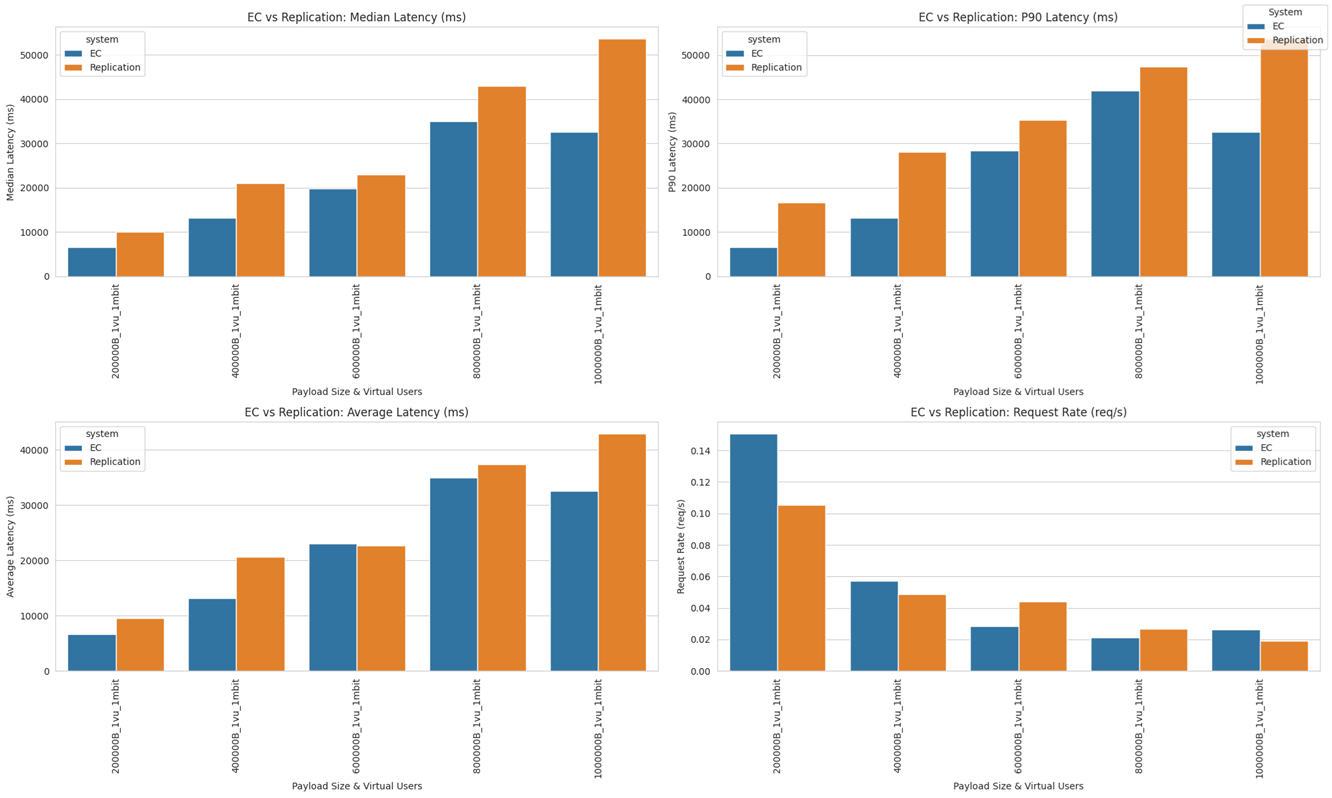
\includegraphics[width=\columnwidth]{resources/chapter-4/write_bigload_slownet.png}
    \caption{Write Performance on Low Bandwidth with Large Payload}
    \label{fig:write-performance-comparison}
\end{figure}

\subsubsection{Mathematical Performance Modeling}

To precisely determine the performance crossover points, we conducted regression analysis using ridge regression to model the relationship between bandwidth, payload size, and response time. The resulting three-dimensional performance model reveals the boundary conditions where erasure coding outperforms replication.

\begin{figure}[ht]
    \centering
    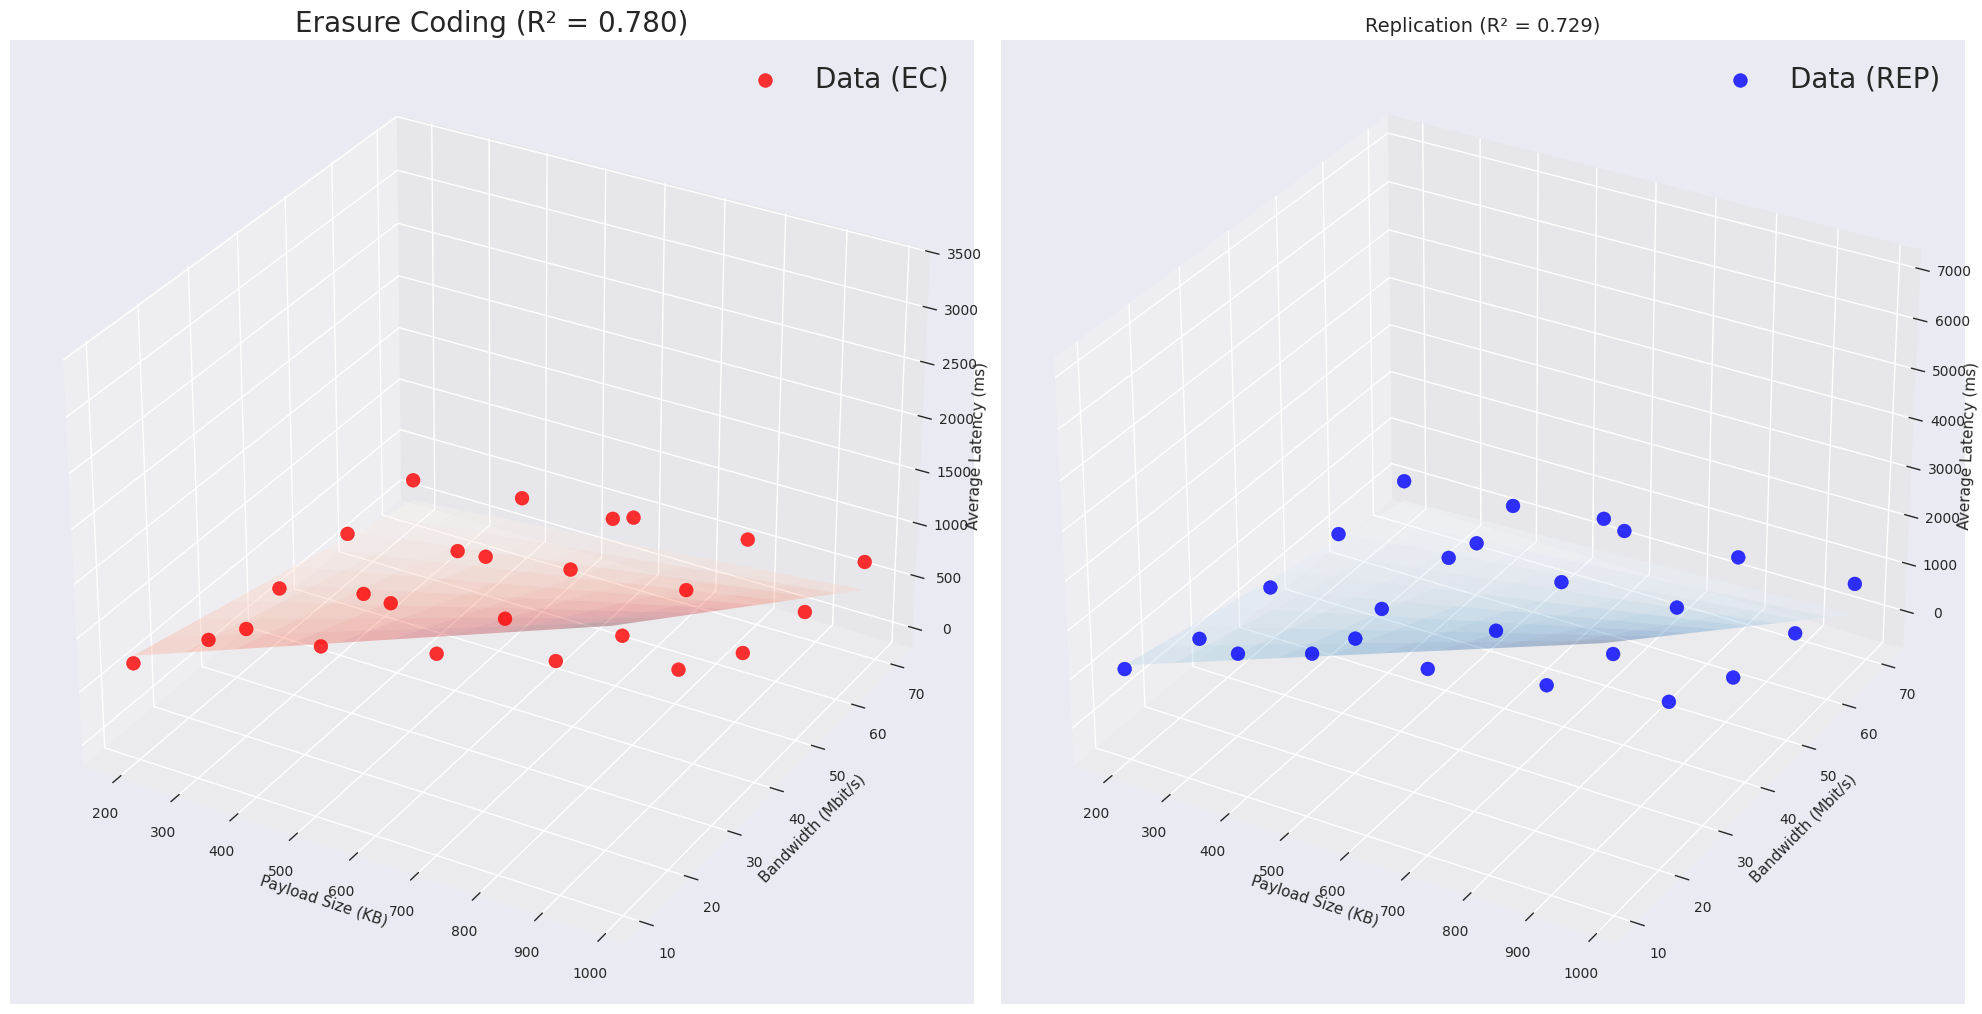
\includegraphics[width=\columnwidth]{resources/chapter-4/write_bigload_avgnet_regression.png}
    \caption{Three-Dimensional Performance Model for Write Operations}
    \label{fig:write-regression-model}
\end{figure}

\subsubsection{Performance Boundary Analysis}

Figure \ref{fig:performance-boundary} presents the derived performance boundary curve, which mathematically defines the threshold conditions. Points above the curve indicate scenarios where erasure coding outperforms replication, while points below favor replication. This boundary demonstrates that erasure coding becomes advantageous when:
\begin{itemize}
\item Network bandwidth is limited ($\leq$10Mbps for payloads $\geq$500KB)
\item Payload size is sufficiently large relative to available bandwidth
\item The ratio of encoding overhead to transmission time reduction favors erasure coding
\end{itemize}

\begin{figure}[ht]
    \centering
    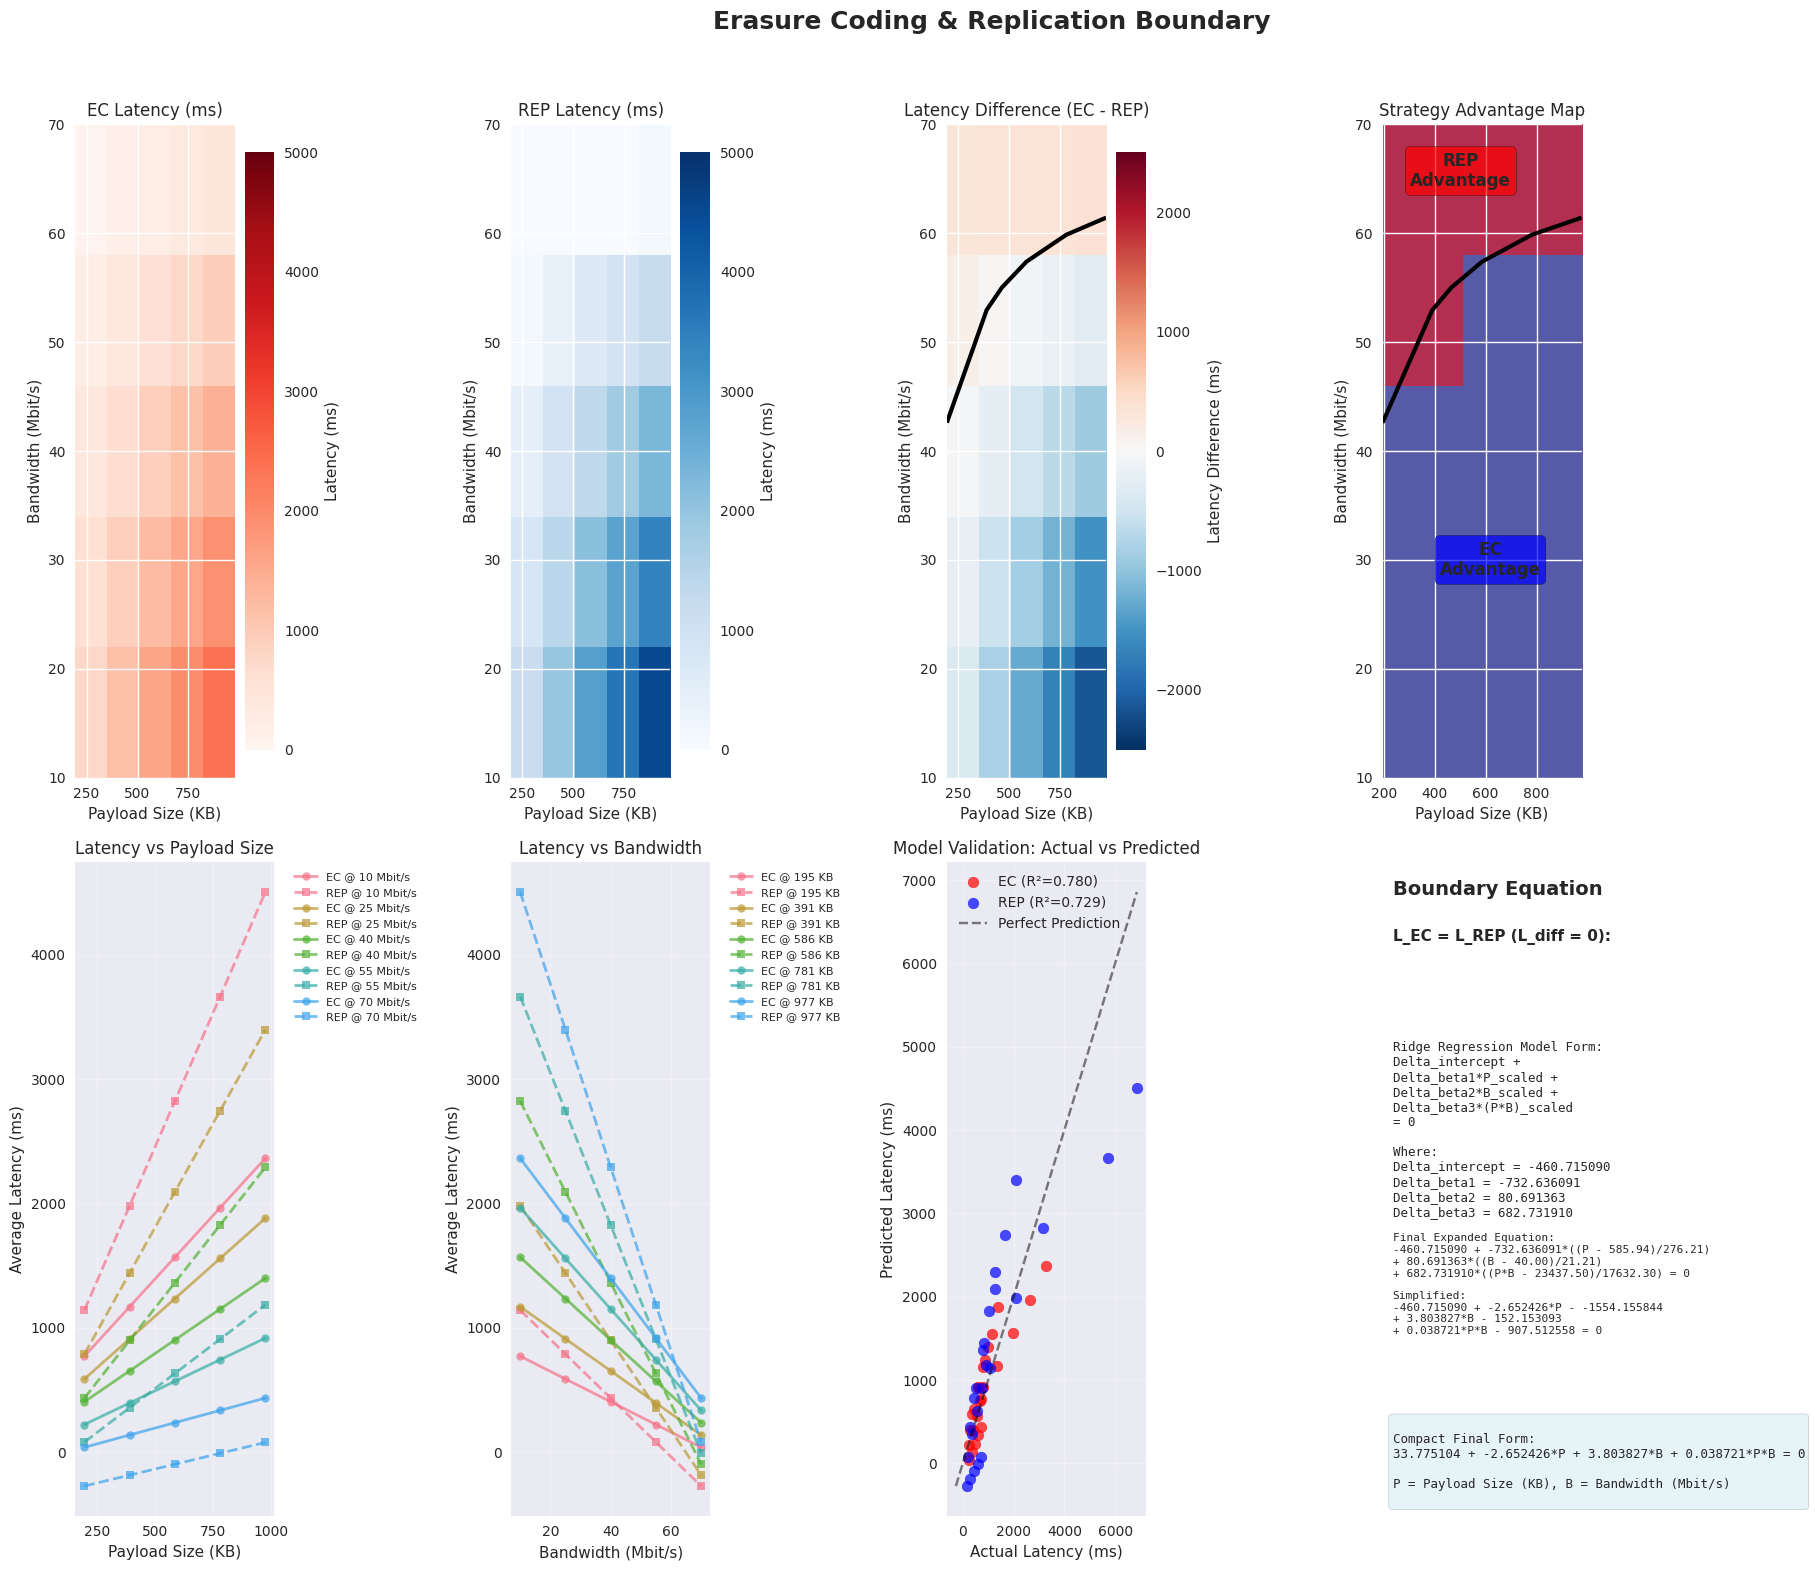
\includegraphics[width=\columnwidth]{resources/chapter-4/write_bigload_avgnet_boundary.png}
    \caption{Performance Boundary Analysis Between Erasure Coding and Replication}
    \label{fig:performance-boundary}
\end{figure}

\subsubsection{Performance Heatmap Visualization}

The comprehensive performance analysis across varying bandwidth and payload combinations is visualized in Figure \ref{fig:write-heatmap}. Blue regions indicate erasure coding superiority, while red regions show replication advantages. This visualization clearly demonstrates the parameter space where each approach excels.

\begin{figure}[ht]
    \centering
    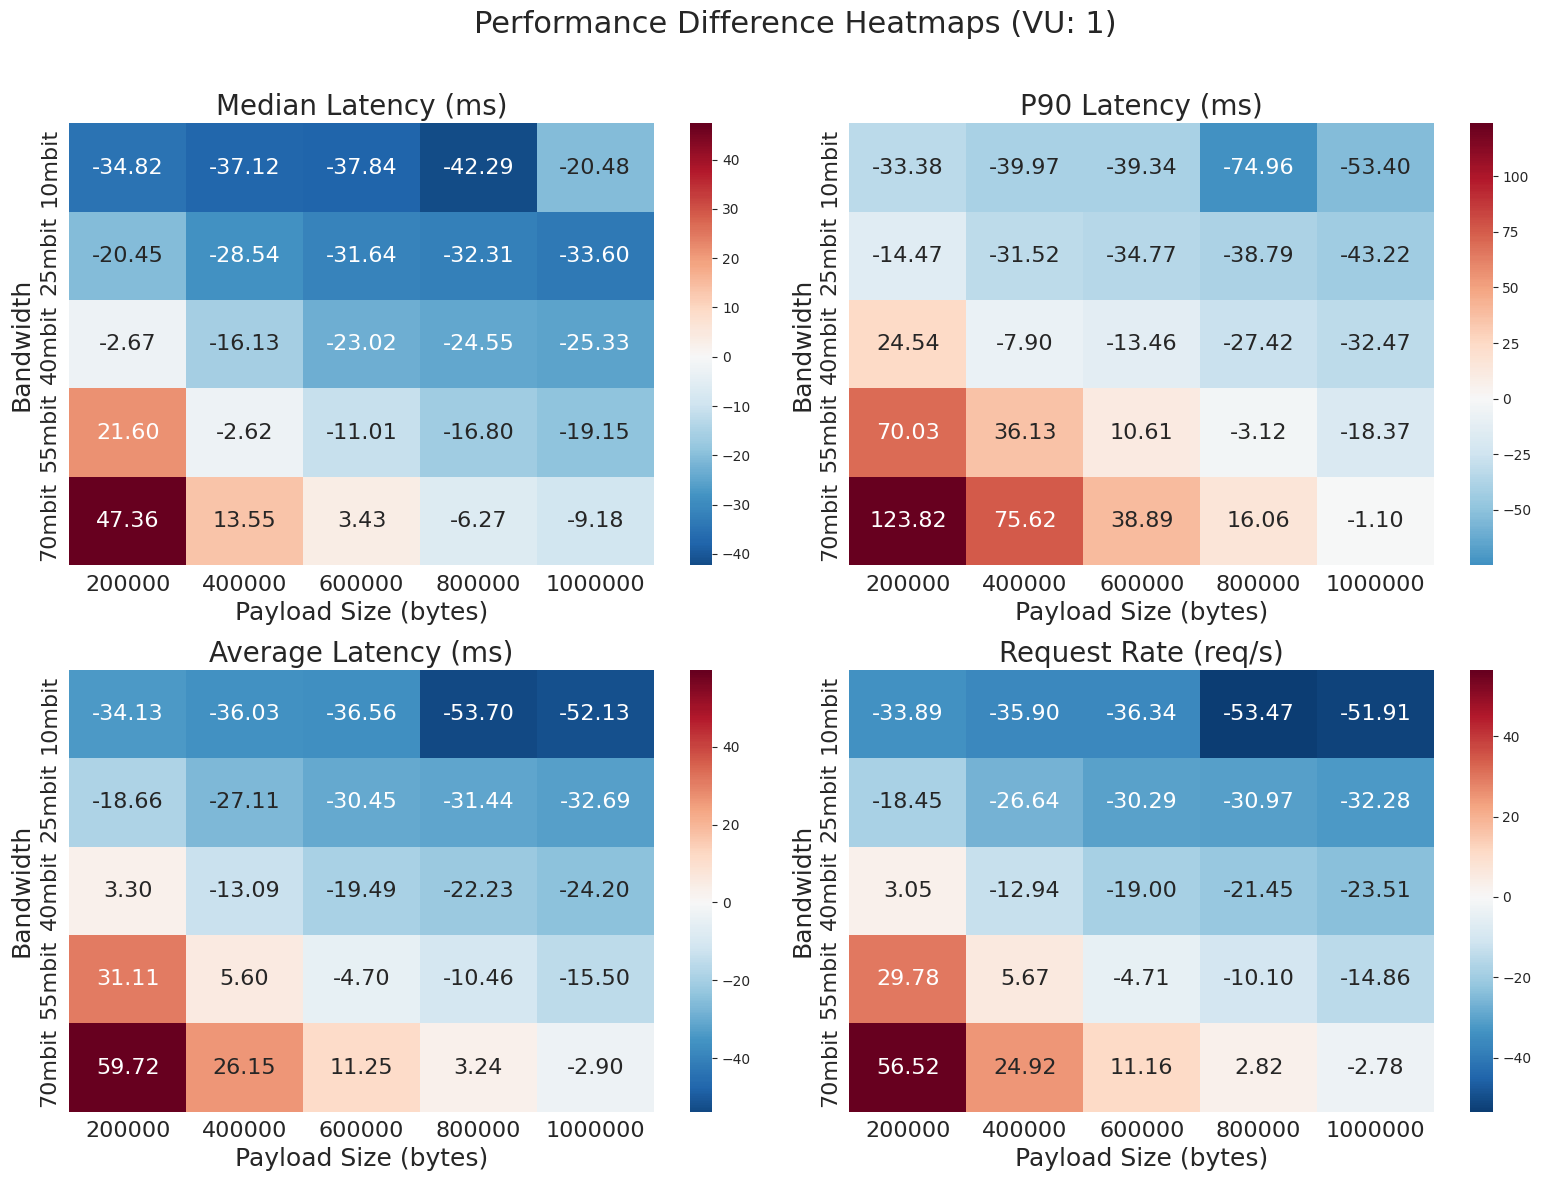
\includegraphics[width=\columnwidth]{resources/chapter-4/write_bigload_avgnet_heatmap.png}
    \caption{Performance Heatmap: Erasure Coding vs Replication for Write Operations}
    \label{fig:write-heatmap}
\end{figure}

\subsection{Read Operation Performance}

For read operations, replication consistently outperforms erasure coding across all tested parameter combinations. This performance difference is mathematically proven through latency analysis.

\subsubsection{Mathematical Latency Analysis}

The latency for erasure coded reads can be expressed as:
\begin{equation}
L_{EC} = T_{data} + T_{reconstruction} + T_{shard}
\label{eq:ec-read-latency}
\end{equation}

While replication read latency is simply:
\begin{equation}
L_{REP} = T_{data}
\label{eq:rep-read-latency}
\end{equation}

The performance difference is therefore:
\begin{equation}
\Delta L = L_{EC} - L_{REP} = T_{reconstruction} + T_{shard}
\label{eq:read-latency-diff}
\end{equation}

This fundamental difference ensures that replication will always outperform erasure coding for read operations, as reconstruction and shard retrieval operations add unavoidable overhead.

\begin{figure}[ht]
    \centering
    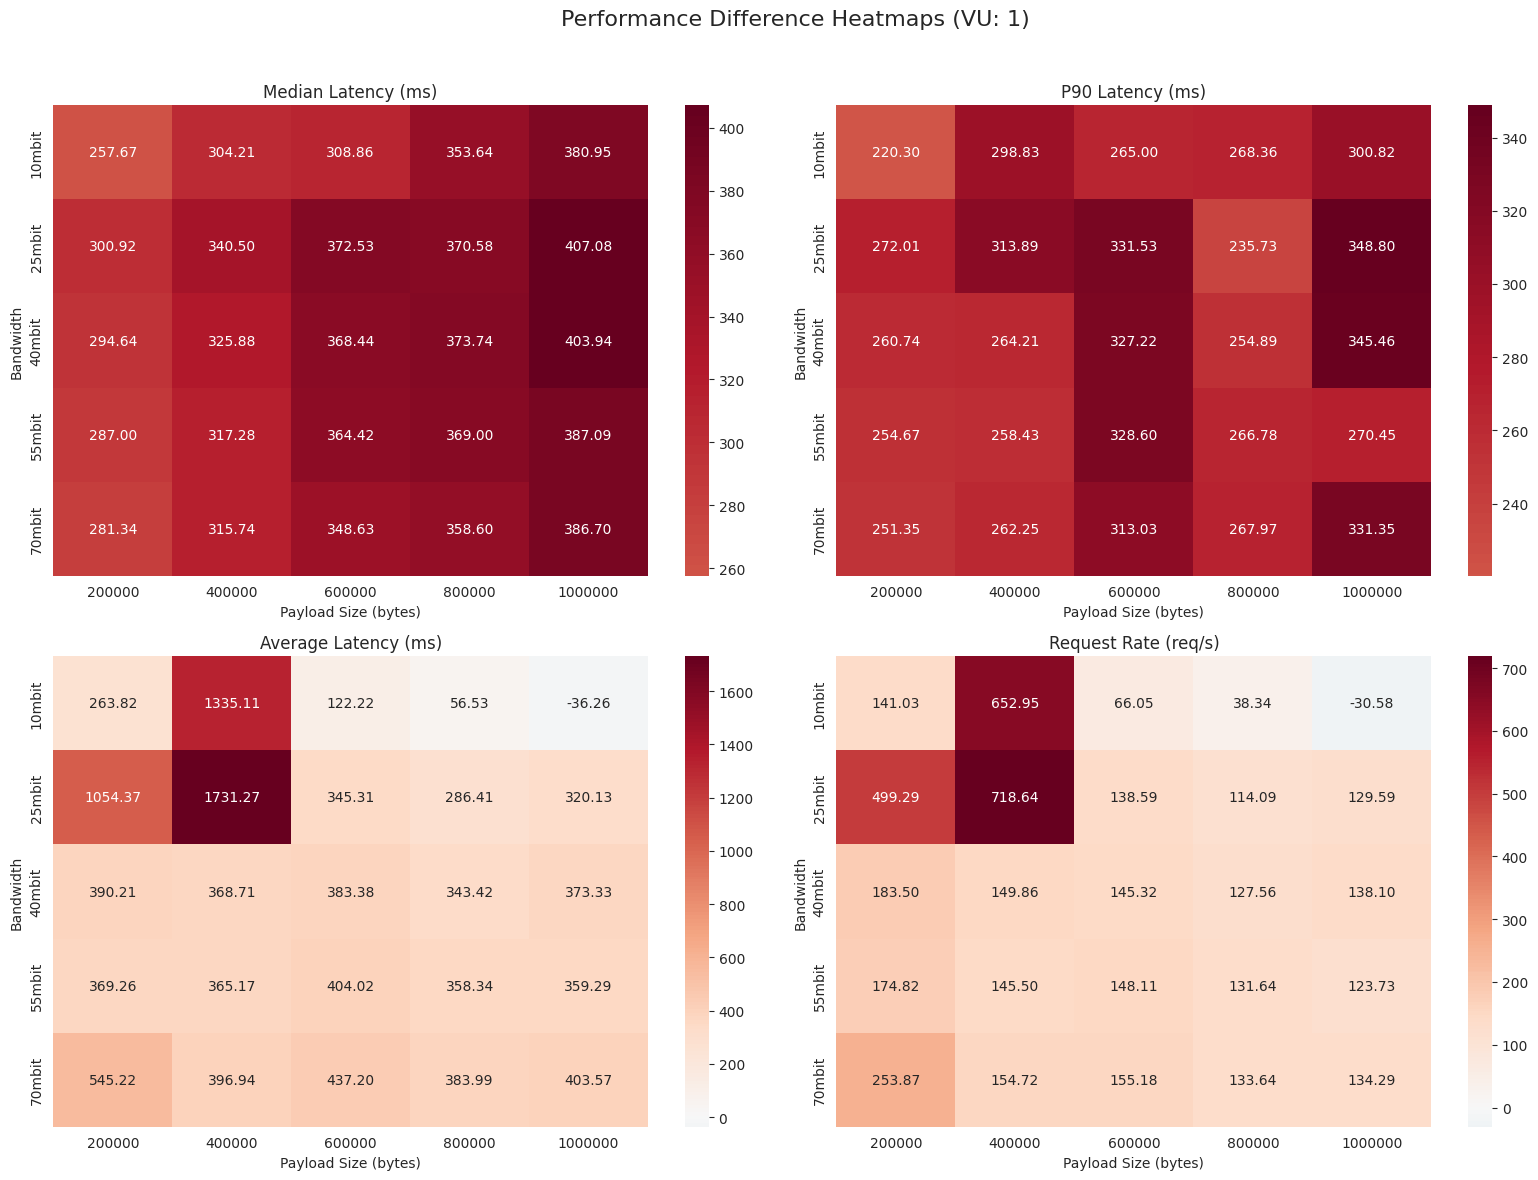
\includegraphics[width=\columnwidth]{resources/chapter-4/read_bigload_avgnet_heatmap.png}
    \caption{Read Performance Heatmap Showing Consistent Replication Advantage}
    \label{fig:read-heatmap}
\end{figure}

\subsubsection{Impact of In-Memory Caching}

The implementation includes an in-memory store that can mitigate read performance penalties. With caching, the effective erasure coding read latency becomes:
\begin{equation}
L_{EC} = T_{data} + (T_{reconstruction} + T_{shard}) \times (1 - \text{hit rate})
\label{eq:ec-read-latency-cached}
\end{equation}

This demonstrates that high cache hit rates can significantly reduce the performance gap, though replication maintains its fundamental advantage.

\subsection{Storage Efficiency}

Erasure coding demonstrates significant advantages in storage efficiency. This storage efficiency becomes particularly valuable in large-scale deployments where storage costs are significant.

\section{Discussion}

\subsection{Theoretical Framework and Practical Implications}

The research establishes a theoretical framework for understanding the performance trade-offs between erasure coding and replication in distributed key-value stores. The mathematical modeling reveals that the performance crossover is fundamentally governed by the relationship between computational overhead and network transmission efficiency.

The derived performance boundary curve provides practical guidance for system architects. Erasure coding is most suitable for distributed key-value store databases operating under specific conditions:
\begin{itemize}
\item Large data objects (>500KB) where encoding overhead is amortized
\item Limited network bandwidth environments (<10Mbps)
\item Write-heavy workloads where storage efficiency is critical
\item Geographically distributed systems with high inter-node latency
\item Cost-sensitive deployments prioritizing storage optimization
\end{itemize}

\subsection{System Design Considerations}

The analysis reveals several critical design considerations:

\textbf{Adaptive System Architecture}: The clear delineation of performance boundaries suggests that adaptive systems could dynamically switch between erasure coding and replication based on real-time workload characteristics, data size patterns, and network conditions.

\textbf{Caching Strategy}: The mathematical analysis of in-memory caching demonstrates that strategic caching can significantly mitigate read performance penalties in erasure coded systems. Systems with predictable access patterns could leverage high cache hit rates to approach replication performance for reads while maintaining erasure coding benefits for writes.

\textbf{Workload Characterization}: The fundamental performance differences between read and write operations suggest that workload characterization is crucial for system optimization. Write-heavy workloads with large objects benefit most from erasure coding, while read-heavy workloads favor replication.

\subsection{Broader Implications for Distributed Systems}

The findings have broader implications beyond key-value stores:

\textbf{Edge Computing}: In edge computing scenarios with limited bandwidth to central data centers, erasure coding provides both performance and storage benefits for large data synchronization tasks.

\textbf{IoT Data Management}: Internet of Things applications generating large sensor data payloads can benefit from erasure coding when transmitting over constrained networks.

\textbf{Backup and Archival Systems}: Long-term storage systems handling large files benefit significantly from erasure coding's storage efficiency while tolerating higher read latencies.

\subsection{Limitations and Model Validity}

The current implementation and analysis have several important limitations:

\textbf{Static Configuration}: The erasure coding implementation uses fixed parameters (data and parity shards), limiting adaptability to varying workload characteristics.

\textbf{Environmental Constraints}: The regression model is valid only under the specific experimental conditions and hardware configurations tested. Different computational capabilities, memory speeds, or network characteristics would require model recalibration.

\textbf{Simplified Workload}: The analysis focuses solely on read and write operations without considering complex transaction patterns, consistency requirements, or failure scenarios that occur in production systems.

\textbf{Network Simulation}: Testing was conducted in controlled virtual environments with simulated network conditions, which may not fully capture the complexity and variability of real-world network behavior.

\section{Conclusion}

This research provides a comprehensive performance analysis of erasure coding versus replication in distributed key-value store databases, establishing both theoretical foundations and practical guidelines for system design decisions. The analysis demonstrates that the choice between erasure coding and replication is not binary but depends on a complex interplay of system characteristics, workload patterns, and performance requirements.

\subsection{Key Results}

\begin{itemize}
\item \textbf{Write performance}: Erasure coding has an advantage for write operations when data objects are large and network bandwidth is low. In distributed key-value stores dominated by small objects, erasure coding is applicable only in the special case of sufficiently large objects and limited bandwidth; otherwise replication is preferable.
\item \textbf{Conditions for write improvement}: Based on the analysis, erasure-coded write response time is lower than replication when bandwidth and payload size for write operations are sufficiently large. No tested condition showed erasure coding outperforming replication for read operations.
\item \textbf{Storage efficiency}: For use cases with large objects, erasure coding reduces stored data volume compared to replication and thus reduces storage cost.
\end{itemize}

\subsection{Future Research Directions}

The research suggests several avenues for future investigation:

\begin{itemize}
\item \textbf{Recovery Analysis}: Erasure coding has a different recovery model compared to replication, which may impact performance and fault tolerance. Future work could explore the trade-offs involved in recovery strategies for both approaches.
\item \textbf{Additional Variables}: Future research could investigate other variables that impact the performance of erasure coding and replication, such as system configurations, hardware performance impacts, and system architecture.
\item \textbf{Hybrid Systems}: Development of systems that combines erasure coding and replication based on workload characteristics, network conditions, and performance requirements.
\item \textbf{Erasure Coding Optimizations}: The exploration of advanced erasure coding techniques, such as locally repairable codes and adaptive coding strategies, to enhance performance and reduce overhead.
\item \textbf{Real-world Validation}: Validation in actual production environments to verify the analysis result under real-world conditions with complex failure patterns and varying workloads.
\end{itemize}

The implementation and experimental artifacts are available in the project's open-source repository \cite{ajiw2025distkv}.